%!TEX program = xelatex+makeindex+bibtex
\documentclass[final]{scrreprt} %scrreprt of scrartcl
% Include all project wide packages here.
\usepackage{fullpage}
\usepackage{polyglossia}
\setmainlanguage{english}
\usepackage{csquotes}
\usepackage{graphicx}
\usepackage{epstopdf}
\usepackage{pdfpages}
\usepackage{caption}
\usepackage[list=true]{subcaption}
\usepackage{float}
\usepackage{standalone}
\usepackage{import}
\usepackage{tocloft}
\usepackage{wrapfig}
\usepackage{authblk}
\usepackage{array}
\usepackage{booktabs}
\usepackage[toc,page,title,titletoc]{appendix}
\usepackage{xunicode}
\usepackage{fontspec}
\usepackage{pgfplots}
\usepackage{SIunits}
\usepackage{units}
\pgfplotsset{compat=newest}
\pgfplotsset{plot coordinates/math parser=false}
\newlength\figureheight 
\newlength\figurewidth
\usepackage{amsmath}
\usepackage{mathtools}
\usepackage{unicode-math}
\usepackage[
    backend=bibtexu,
	texencoding=utf8,
bibencoding=utf8,
    style=ieee,
    sortlocale=en_US,
    language=auto
]{biblatex}
\usepackage{listings}
\newcommand{\includecode}[3][c]{\lstinputlisting[caption=#2, escapechar=, style=#1]{#3}}
\newcommand{\superscript}[1]{\ensuremath{^{\textrm{#1}}}}
\newcommand{\subscript}[1]{\ensuremath{_{\textrm{#1}}}}


\newcommand{\chapternumber}{\thechapter}
\renewcommand{\appendixname}{Bijlage}
\renewcommand{\appendixtocname}{Bijlagen}
\renewcommand{\appendixpagename}{Bijlagen}

\usepackage[hidelinks]{hyperref} %<--------ALTIJD ALS LAATSTE

\renewcommand{\familydefault}{\sfdefault}

\setmainfont[Ligatures=TeX]{Myriad Pro}
\setmathfont{Asana Math}
\setmonofont{Lucida Console}

\usepackage{titlesec, blindtext, color}
\definecolor{gray75}{gray}{0.75}
\newcommand{\hsp}{\hspace{20pt}}
\titleformat{\chapter}[hang]{\Huge\bfseries}{\chapternumber\hsp\textcolor{gray75}{|}\hsp}{0pt}{\Huge\bfseries}
\renewcommand{\familydefault}{\sfdefault}
\renewcommand{\arraystretch}{1.2}
\setlength\parindent{0pt}

%For code listings
\definecolor{black}{rgb}{0,0,0}
\definecolor{browntags}{rgb}{0.65,0.1,0.1}
\definecolor{bluestrings}{rgb}{0,0,1}
\definecolor{graycomments}{rgb}{0.4,0.4,0.4}
\definecolor{redkeywords}{rgb}{1,0,0}
\definecolor{bluekeywords}{rgb}{0.13,0.13,0.8}
\definecolor{greencomments}{rgb}{0,0.5,0}
\definecolor{redstrings}{rgb}{0.9,0,0}
\definecolor{purpleidentifiers}{rgb}{0.01,0,0.01}


\lstdefinestyle{csharp}{
language=[Sharp]C,
showspaces=false,
showtabs=false,
breaklines=true,
showstringspaces=false,
breakatwhitespace=true,
escapeinside={(*@}{@*)},
columns=fullflexible,
commentstyle=\color{greencomments},
keywordstyle=\color{bluekeywords}\bfseries,
stringstyle=\color{redstrings},
identifierstyle=\color{purpleidentifiers},
basicstyle=\ttfamily\small}

\lstdefinestyle{c}{
language=C,
showspaces=false,
showtabs=false,
breaklines=true,
showstringspaces=false,
breakatwhitespace=true,
escapeinside={(*@}{@*)},
columns=fullflexible,
commentstyle=\color{greencomments},
keywordstyle=\color{bluekeywords}\bfseries,
stringstyle=\color{redstrings},
identifierstyle=\color{purpleidentifiers},
}

\lstdefinestyle{matlab}{
language=Matlab,
showspaces=false,
showtabs=false,
breaklines=true,
showstringspaces=false,
breakatwhitespace=true,
escapeinside={(*@}{@*)},
columns=fullflexible,
commentstyle=\color{greencomments},
keywordstyle=\color{bluekeywords}\bfseries,
stringstyle=\color{redstrings},
identifierstyle=\color{purpleidentifiers}
}

\lstdefinestyle{vhdl}{
language=VHDL,
showspaces=false,
showtabs=false,
breaklines=true,
showstringspaces=false,
breakatwhitespace=true,
escapeinside={(*@}{@*)},
columns=fullflexible,
commentstyle=\color{greencomments},
keywordstyle=\color{bluekeywords}\bfseries,
stringstyle=\color{redstrings},
identifierstyle=\color{purpleidentifiers}
}

\lstdefinestyle{xaml}{
language=XML,
showspaces=false,
showtabs=false,
breaklines=true,
showstringspaces=false,
breakatwhitespace=true,
escapeinside={(*@}{@*)},
columns=fullflexible,
commentstyle=\color{greencomments},
keywordstyle=\color{redkeywords},
stringstyle=\color{bluestrings},
tagstyle=\color{browntags},
morestring=[b]",
  morecomment=[s]{<?}{?>},
  morekeywords={xmlns,version,typex:AsyncRecords,x:Arguments,x:Boolean,x:Byte,x:Char,x:Class,x:ClassAttributes,x:ClassModifier,x:Code,x:ConnectionId,x:Decimal,x:Double,x:FactoryMethod,x:FieldModifier,x:Int16,x:Int32,x:Int64,x:Key,x:Members,x:Name,x:Object,x:Property,x:Shared,x:Single,x:String,x:Subclass,x:SynchronousMode,x:TimeSpan,x:TypeArguments,x:Uid,x:Uri,x:XData,Grid.Column,Grid.ColumnSpan,Click,ClipToBounds,Content,DropDownOpened,FontSize,Foreground,Header,Height,HorizontalAlignment,HorizontalContentAlignment,IsCancel,IsDefault,IsEnabled,IsSelected,Margin,MinHeight,MinWidth,Padding,SnapsToDevicePixels,Target,TextWrapping,Title,VerticalAlignment,VerticalContentAlignment,Width,WindowStartupLocation,Binding,Mode,OneWay,xmlns:x}
}

%defaults
\lstset{
basicstyle=\ttfamily\small,
extendedchars=false,
numbers=left,
numberstyle=\ttfamily\tiny,
stepnumber=1,
tabsize=4,
numbersep=5pt
}
\addbibresource{../../library/bibliography.bib}
\usepackage{amsmath}
\usepackage{graphicx}
\title{Module 3 - Report}
\author{Alex {Misdorp} \and Sander {van Dijk}}
\begin{document}

\chapter{Assignment 2}
\section*{Task 3: Identifying the models' parameters}
\section*{Task 4: Observer Design}
In order to get accurate information about the velocity of the car, an observer is constructed. The poles were chosen to be X and Y, the reason being: ...... From here on we calculated the L matrix which turned out to be:
\begin{equation}
\centering
L =
\begin{bmatrix}
  -1,218 & -0.170
\end{bmatrix}
\end{equation}

We applied the L matrix to our simulation to create an observer which can be seen in figure \ref{fig:simcircuit}.

\begin{figure}[h!]
\centering
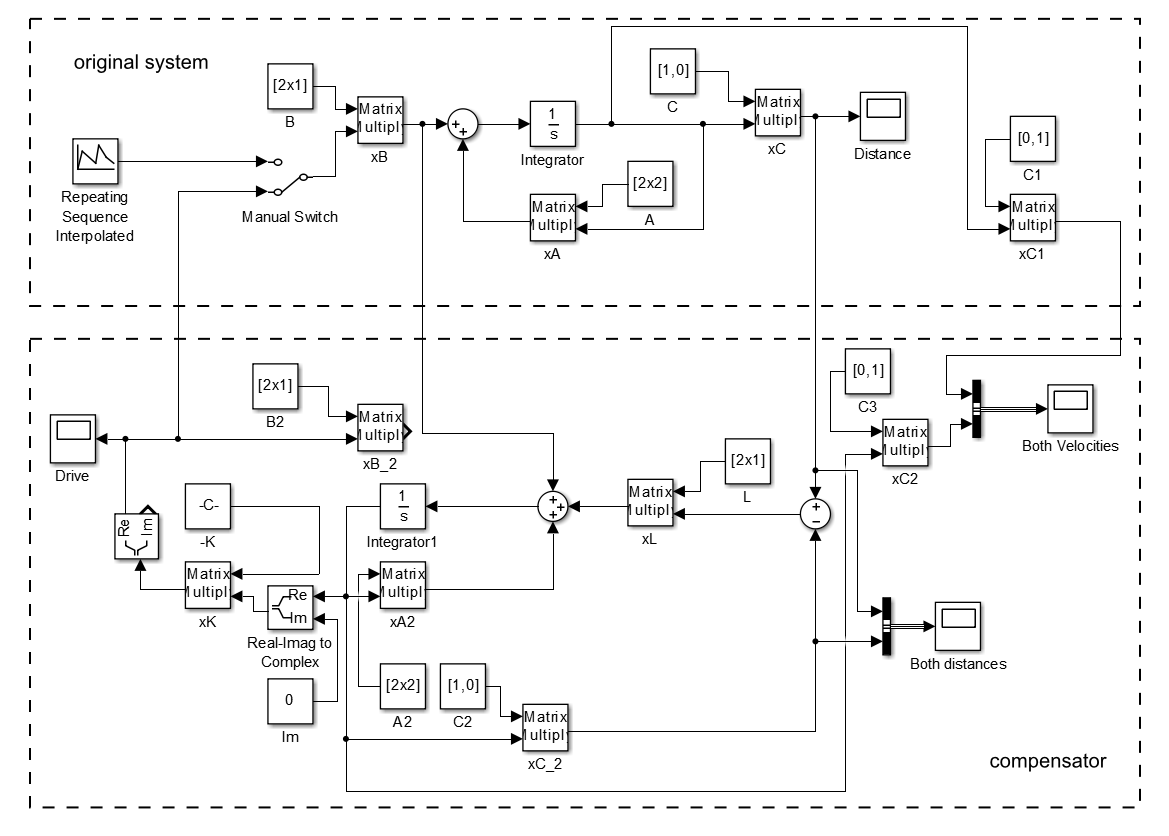
\includegraphics[width=\linewidth]{res/model-rest.png}
\caption{Model used for simulation.}
\label{fig:simcircuit}
\end{figure}

As a result the observer tracks the velocity fairly well. This can be seen in figure \ref{fig:observer} where the pink line represent the actual velocity and the blue line the observed velocity. 

\begin{figure}[h!]
\centering
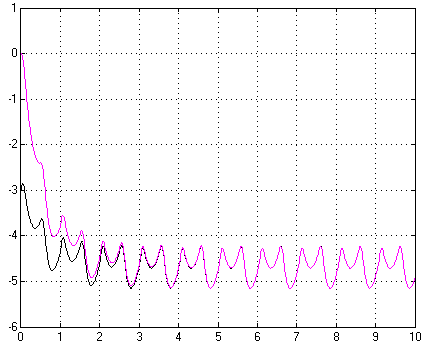
\includegraphics[width=\linewidth]{res/observer-res.png}
\caption{Observer in werking.}
\label{fig:simcircuit}
\end{figure}

After about 1,5 seconds there is only a slight difference between the two lines and after two seconds they are nearly identical. This is in agreement with the requirements for an observer; the difference $x(t)-\hat{x}$ converges to zero and after a certain time point $t_i$ where $x(t) = \hat{x}$, this equation remains satisfied for $t$\geq $t_i$.

\section*{Task 5: Controller design}

To obtain oscillatory behavior we chose poles at X and Y. This results in the following K matrix:
\begin{equation}
\centering
K = 
\begin{bmatrix}
  XXX & XXX
\end{bmatrix}
\end{equation}
Leading to the oscillatory response as seen in figure \ref{fig:oscillatory}.

\begin{figure}[h!]
\centering
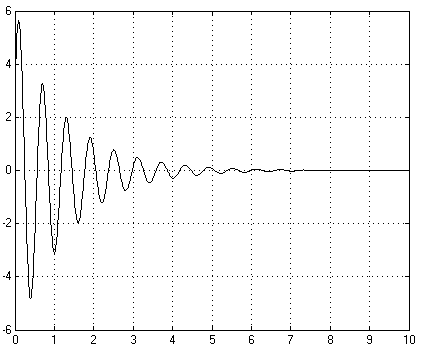
\includegraphics[scale = 0.5]{res/osc2-res.png}
\caption{Oscillatory behaviour.}
\label{fig:oscillatory}
\end{figure}

To obtain the desired critically damped response we had to choose our poles in the left half-plane. One would not want the poles to be too close to zero which might cause stability issues, on the other hand one would not want to place the poles too far to the left because this might not be practically feasible. Therefore we chose our poles at $-1+100i$ and $1+101i$. This results in the following K matrix:
\begin{equation}
\centering
K =
\begin{bmatrix}
  0 & 0,8
\end{bmatrix}
\end{equation}

Using this K matrix we receive a critically damped response as seen in figure \ref{fig:critically}.

\begin{figure}[H]
\centering
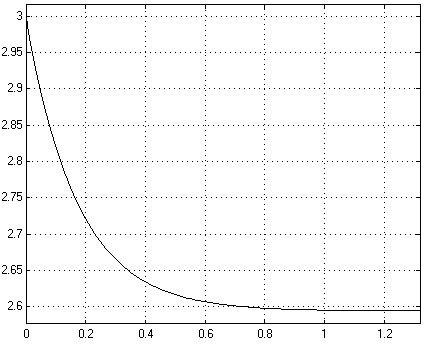
\includegraphics[scale = 0.5]{res/critically-res.png}
\caption{Critically damped behaviour.}
\label{fig:critically}
\end{figure}

In accordance to the preceding figure we obtain the desired closed loop behaviour in our simulation.\\\\
\\
CONTROL INPUT ontbreekt nog???\\
welke polen???\\
dingen voor assignment 1 en 2\\
\end{document}